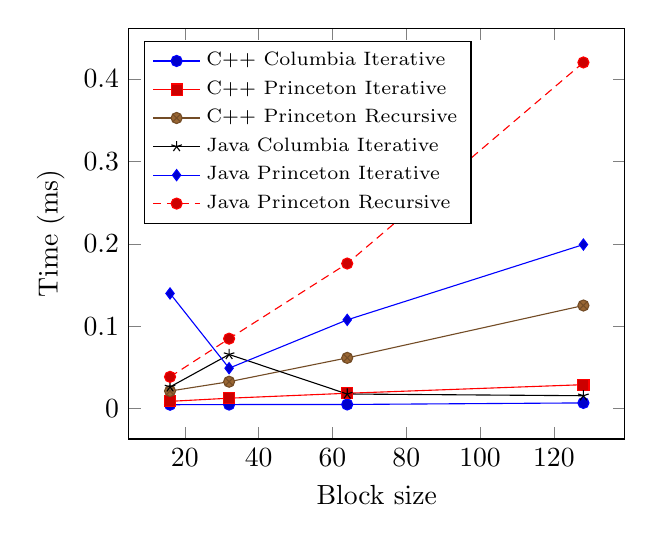
\begin{tikzpicture}
\begin{axis}[xlabel={Block size},ylabel={Time (ms)},width=0.65\linewidth,legend pos=north west,scaled y ticks = false,legend cell align=left,legend style={font=\scriptsize}]
\addplot coordinates {
(16, 0.0049)
(32, 0.0051)
(64, 0.0052)
(128, 0.0071)
};
\addplot coordinates {
(16, 0.0090)
(32, 0.0128)
(64, 0.0188)
(128, 0.0292)
};
\addplot coordinates {
(16, 0.0215)
(32, 0.0328)
(64, 0.0617)
(128, 0.1252)
};
\addplot coordinates {
(16, 0.0265)
(32, 0.0658)
(64, 0.0179)
(128, 0.0158)
};
\addplot coordinates {
(16, 0.1398)
(32, 0.0492)
(64, 0.1078)
(128, 0.1991)
};
\addplot coordinates {
(16, 0.0387)
(32, 0.0850)
(64, 0.1761)
(128, 0.4199)
};
\legend{C++ Columbia Iterative,C++ Princeton Iterative,C++ Princeton Recursive,Java Columbia Iterative,Java Princeton Iterative,Java Princeton Recursive}
\end{axis}
\end{tikzpicture}
